\documentclass[11pt]{article}
\usepackage{amsmath}
\usepackage{fullpage}
\usepackage{framed}
\usepackage{color}
\usepackage{graphicx}
\usepackage[backref,colorlinks,linkcolor=blue,citecolor=blue]{hyperref}
\usepackage{parskip}

\definecolor{shadecolor}{rgb}{0.757, 0.882, 0.925}

\begin{document}

Dr. Athanasios Chantis\hfill{\today}\\
Assistant Editor\\
Physical Review B

Dear Dr. Athanasios Chantis,\\

Please find here enclosed the revised version of the manuscript
BP12969/Anderson.

We thank the referees for their positive and useful comments and suggestions of
our manuscript and we believe that it helped us to improve the quality of our
work.

In the following, we answer all the points raised by the referees and we also
list all the changes made in the paper. In the \verb=pdf=  version we have put
in red the changes for easy reference. Below, our responses are enclosed in blue
boxes.

We are confident that all suggestions have been met, and hope that our
manuscript can now be published in Physical Review B.


\section{Report of the First Referee -- BP12969/Anderson}

Anderson and colleagues present a follow up to their PRB 2015 paper [Ref. 19]
which described a theoretical framework that allows quantitative calculation of
surface second harmonic generation at the independent particle level. The main
concepts treated in that work - scissors shift, nonlocal terms in the matrix
elements, and a slab cut function, within a single formulation - are
demonstrated here by means of ab initio calculations on Si(111)-(1x1):H and
compared with various experimental data. In addition, the authors report on
other technical aspects such as three vs two layer models and sensitivity to
atomic geometry. The text is very well written and easy to read. The theory
section repeats only the essential formulae of Ref 19, but otherwise reports no
new theoretical development beyond what is reported in e.g. Refs 19 and 24-27.
The calculations and conclusions deserve publication in some form, since
practical SSHG calculations beyond the IP level remain out of reach for most
systems and researchers in the near future, but I consider it a borderline work
for PRB. In the following, I raise some issues that should nonetheless be
addressed.

\begin{enumerate}

\item
One interesting demonstration in Ref. 19 was the sensitivity of computed spectra
(both lineshape and energy) to the chosen value of the scissors shift. There,
the authors used 0.5 and 0.63 eV for clean Si(100)-(2x1), but here they use 0.7
eV for Si(111)-(1x1):H as taken from a published GW calculation. Since the
authors neglect temperature, local field, and excitonic effects, this choice is
somewhat arbitrary. However, they cannot claim such good agreement with
experiment unless they show such a comparison again here (at least for one
dataset). The authors should also comment on why GW eigenvalues/transition
energies are appropriate here, when in linear optics the GW+BSE transition
energies are needed.
\begin{shaded}\label{ref1.01}
The value of the scissors shift comes from GW calculations and depends on the
surface of the material (see Refs 65, 66, and 67 from our previous work for the
clean Si(100)(2x1) surface). It turns out that the scissors value for the clean
Si(100)(2x1) surface is smaller, due to the presence of the surface states. For
linear optics and SHG, GW transition energies are needed. Doing a Bethe-Salpeter
calculation for SSHG will improve the position and the amplitude of the peaks,
but is far beyond the present possibilities. Therefore, we did not adjust the
value of the scissors shift as we want to keep our calculation at the ab initio
level.

We have added a discussion on the scissors shift and the $GW$ and the $GW$+BSE
transition energies in the paragraph just before the Conclusions, and Ref. 53 in
connection to this.
\end{shaded}

\item
Related to this, I find that the authors overinterpret their results and
frequently overstate the agreement with experiment. For instance:

\begin{itemize}

\item 
Page 5: ``relaxed coordinates have an improved peak position''. Can the authors
really claim that agreement is improved, in light of the IP approximation used?
\begin{shaded}\label{ref1.02}
The results presented in Fig. 2 are compared to low-temperature measurements and
correspond to an in-plane susceptibility for which the local-field effects are
expected to be small (see point 8 below for more details). However, we have
changed the sentence to ``$\dots$relaxed coordinates have a peak
position$\dots$''
\end{shaded}

\item
The authors on Page 6 refer to Ref. 46, Dadap PRB 1996 for ``It is well known
that temperature causes shifting in the peak position of SHG spectra''. That
work does not discuss temperature. I believe the authors intended to refer to
Dadap PRB 56 13367 (1997), which shows several spectra redshifting with higher
T. Hence ``Low temperature measurements for the SHG yield will lead to more
closely matched results'' does not seem to be correct - quite the opposite.
\begin{shaded}\label{ref1.03}
Indeed, we cited the wrong article; it is now correctly cited. It is worth
noting that the correct article, PRB 56, 13367 (1997), concerns
$\mathcal{R}_{pP}$ from a different surface altogether. $\mathcal{R}_{pS}$ from
the Si(111)(1$\times$1):H surface may not behave in the same way.
 
We have modified the text accordingly in the fourth paragraph in Sec. V B, page
6. We have also added some discussion along the same lines for
$\mathcal{R}_{pP}$ in first paragraph of Sec. V D, page 8.
\end{shaded}

\item
Page 6: ``the three layer model best reproduces both the lineshape and 
intensity'' is again somewhat generous, since the bulk/2L spectra have near
identical lineshapes (``mostly consistent'', as written on page 7). Such a
conclusion might be valid after Fig. 7.
\begin{shaded}\label{ref1.04}
We have changed ``Ultimately, the three layer model best reproduces both the
lineshape and intensity$\dots$'' to ``Ultimately, the intensity of the three
layer model is the closest to the experiment.''

Also, we have modified the text towards the end of the first paragraph of Sec. V
D, page 8.
\end{shaded}

\item
Page 7: ``inclusion of .. nonlocal part .. gives much better comparison''.
Again, the evidence for this is tiny. I do not doubt that the inclusion is
formally correct, and perhaps for some other material/pseudopotential essential,
but the results presented here do not justify such a strong conclusion.
Furthermore, this point was already well demonstrated in Ref. 19.
\begin{shaded}\label{ref1.05}
We have changed this concluding remark to how it now appears at the end of Sec.
V B, page 7.
\end{shaded}

\item
The few speculative remarks on temperature and oxidation effects on experimental
SSHG spectra does not justify ``Our comparisons also indicate the effects of
temperature and surface adsorption'' in the abstract, although they are
acceptable in the text.
\begin{shaded}\label{ref1.06}
We have removed the specified sentence from the abstract.
\end{shaded}

\begin{shaded}\label{ref1.13}
Besides above points, we have toned down the overstatements regarding the
agreement with experiment.
\end{shaded}

\end{itemize}

\item
In all cases shown, the bulk model yields near identical lineshapes and seems
just as good as the 3L model except for a constant underscaling of about 5. I
suspect this is because the authors chose a passivated surface with no surface
states, so that all features appear around E1 and E2. If the authors repeated
such a comparison using the Si(100)-(2x1) surface (used in Ref 19) they might
demonstrate a clearer difference between 3L and bulk. I think such a comparison
is most important here, even in the absence of experimental data. Secondly: do
the authors' calculations on Si(111)-(1x1):H demonstrate that surface SHG, for a
system without surface states, can be well modeled simply from a bulk
calculation (plus scaling of about ~5) and use of the appropriate formulae? This
seems to be a useful result in itself.
\begin{shaded}\label{ref1.07}
We regret that this might be a misunderstanding due to our naming convention for
the radiation models of $\mathcal{R}_{\mathrm{iF}}$. What we called the {\em
Bulk} model is actually the case for which
$\boldsymbol{\chi}(-2\omega;\omega,\omega)$ radiates from the bulk layer, but
$\boldsymbol{\chi}(-2\omega;\omega,\omega)$ itself is the {\em surface}
nonlinear susceptibility, as it is defined and calculated in the manuscript. If
we were to do a bulk calculation of $\boldsymbol{\chi}(-2\omega;\omega,\omega)$,
we would get zero as  Si is centrosymmetric. We cannot use a bulk calculation of
$\boldsymbol{\chi}(-2\omega;\omega,\omega)$ to model a surface, with or without
surface states.

To correct this possible misunderstanding, we have renamed the three models as:
the 3-layer, the 2-layer-vacuum, and the 2-layer-bulk models; the ``3'' or ``2''
refers to the number of layers, and ``vacuum'' or ``bulk'' refers to the place
from which ${\boldsymbol{\cal P}}(2\omega)$ radiates. We stress the fact that we
always take the surface into account to obatin the susceptibility
$\boldsymbol{\chi}(-2\omega;\omega,\omega)$, otherwise for a bulk system it is
zero.

We have followed the recommendation of the referee, and have analyzed the effect
of the 3 models on the Si(100)(2$\times$1) surface. We agree that, while the
3-layer and the 2-layer-bulk are similar for the Si(111)(1$\times$1):H  surface,
they do not coincide for the Si(100)(2$\times$1) surface. Since the
Si(100)(2$\times$1) surface is another case entirely with limited experimental
data available (without absolute units or covering a wide range of energy), we
consider that including results for this surface it is outside of the scope of
this manuscript.
\end{shaded}

\item
Two broadenings are chosen. These also affect the intensities, of course. The
authors should justify their usage and value (a priori?)
\begin{shaded}\label{ref1.08}
The original idea behind the two different broadenings was that for the
comparison of $\chi_{\parallel\parallel\parallel}(-2\omega;\omega,\omega)$ with
the experiment (Fig. 2), $\sigma=0.05$ eV gives a reasonable result; so we fixed
$\sigma=0.05$ eV for $\chi^{\mathrm{abc}}(-2\omega;\omega,\omega)$. Then, for
${\mathcal R}_{\mathrm{iF}}$ we used $\sigma=0.1$ eV so that the SSHG yield has
a broadening similar to the experimental spectra.

Of course, at this level of approximation there is no a priori value for
$\sigma$ other than trying to find a value that fits well to the experimental
results. We do agree that using two values for $\sigma$ is confusing, so we have
changed all the plots for a unique value of $\sigma=0.075$ eV, where we achieve
an  adequate compromise that is just as good as what we had with the two
different values. For the sake of proving this point, in this reply we show in
Fig. \ref{smearing} the comparison between theoretical results for
$\sigma=0.075$ eV for both $\chi^{\mathrm{abc}}(-2\omega;\omega,\omega)$ and
$\mathcal{R}_{pP}$, along with the ``hybrid'' case where $\sigma=0.05$ eV for
$\chi^{\mathrm{abc}}(-2\omega;\omega,\omega)$ and $\sigma=0.1$ eV for
$\mathcal{R}_{pP}$. We see that qualitatively both approaches give very similar
results. We have added a few sentences about our choice of $\sigma$ in the text
at the end of the Sec. IV, page 5.
\end{shaded}

\begin{figure}[t]
\centering 
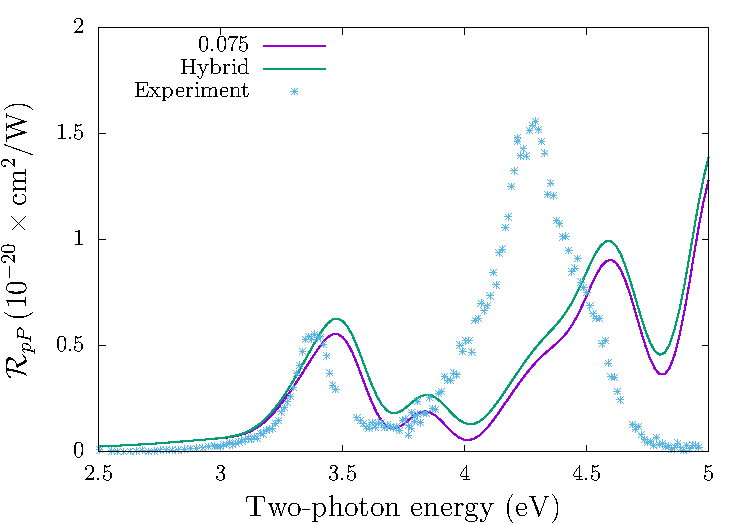
\includegraphics[width=0.55\textwidth]{smearing}
\caption{
(Color online) 
Comparison between theoretical results for 
$\sigma=0.075$ eV for both 
$\chi^{\mathrm{abc}}(-2\omega;\omega,\omega)$ and 
$\mathcal{R}_{pP}$, and the ``hybrid'' case where 
$\sigma=0.05$ eV for 
$\chi^{\mathrm{abc}}(-2\omega;\omega,\omega)$ and 
$\sigma=0.1$ eV for 
$\mathcal{R}_{pP}$. We show  
the experiment for $\mathcal{R}_{pP}$, for 
$\theta=65^{\circ}$. 
\label{smearing}}
\end{figure}

\item
The authors renormalize the surface dielectric function to the volume of the
slab, not the supercell. On page three, they describe the slab as containing
``front, back, subsurface regions...and between these, a bulk region''. Would it
not be more precise, therefore, to renormalize to the volume of the surface
region? Or the half slab? This point is not clear.
\begin{shaded}\label{ref1.09}
The sentence containing ``front, back, subsurface regions...and between these, a
bulk region'' is indeed confusing, so we have removed it.

The super-cell is composed of two regions, a material slab and a vacuum part.
The surface dielectric function is normalized only to the volume of matter and
not to the super-cell. However, we could have calculated the response of the
half slab only (using the cut-function). It has been checked that the response
of a slab is equal to the average of the two half slabs (see also Refs. 36, 37,
and 38). We have added a remark concerning this at the end of Sec. III, page 4.

The situation is different for the second-order susceptibility. As it is
mandatory to use the cut-function, the susceptibility is normalized to the
half-slab. But the quantities used in Sec. V are surface susceptibilities,
normalized to the surface plane. They are then independent of the height of the
material slab. Therefore, the $\chi^{\mathrm{abc}}(-2\omega;\omega,\omega)$
entering in $\mathcal{R}_{iF}$ are always surface susceptibilities. We have
added some remarks at the end of the left column on page 4.
\end{shaded}

\item
Page 8, ``but with four times less intensity'' should read ``but with eight
times less intensity.''
\begin{shaded}\label{ref1.10}
We have corrected the text, changing ``four'' to ``eight.''
\end{shaded}

\item
The temperature used in the experiments should be noted in each figure caption
(or on the figure), and not only in the text.
\begin{shaded}\label{ref1.11}
The temperature at which the experiment was taken is added at the end of each
figure caption.
\end{shaded}

\item
On page 8, local fields are mentioned as possibly being important for the out of
plane components. A sentence expanding on this (what local fields are and why
they are more important perpendicular to the surface) would help a non expert.
\begin{shaded}\label{ref1.12}
Local fields reveal the inhomogeneities in the material, which are by far more
important perpendicular to the surface than in the plane. This can be evidenced
for Silicon, as Reflectance Anisotropy measurements are well described by ab
initio calculations neglecting local field Effects (see for example, Refs. 51
and 52). It is therefore expected that the component in the plane
($\chi_{\parallel\parallel\parallel}(-2\omega;\omega,\omega)$) will be less
sensitive to the inclusion of local-fields, while it might be important for the
others. Note however that this conclusion may be material-dependent.

We have added a few comments about these effects in the second paragraph of Sec.
V D, page 8.
\end{shaded}

\end{enumerate}



\section{Report of the Second Referee -- BP12969/Anderson}

In this paper an ab initio calculation of surface second-harmonic generation of
Si(111)(1x1):H surface has been carried out using the ABINIT pseudopotential
code for the ground state calculation and the DP code for the calculation of the
nonlinear part of the pseudopotential to the nonlinear susceptibility. Like in
their previous paper (see Ref. 19), they used the independent particle
approximation to include the scissors correction, the contribution of the
nonlocal part of the pseudopotentials, and a cut function to extract the surface
response to the calculation of the nonlinear susceptibility tensor and the
surface second-harmonic generation (SSHG) yield. This work is therefore a
continuation of their previous work published in Phys. Rev. B 91, 075302. In
this work they used their previous results of the nonlinear susceptibility to
calculate the SSHG yield of Si(111)(1x1):H surface and compare the results with
various experiments. The scissors operator used seems to make their calculation
in fair agreement with experiments. However, it is unfortunate that the details
of their derivations of the SSHG yield are put in a paper (Ref. 34), which is
submitted, but the information about the journal is missing. I suppose this is a
mistake. I advise the authors either to put this paper in arXiv.org or to put
the derivation in an appendix or supplementary information. This will be helpful
to the specialized reader. He (she) will be able to fully derive their formulas,
especially when their previous publication of the SSHG yield (PRB 66, 195329)
seems to be incorrect due to errors in their previous formulas.
\begin{shaded}\label{ref2.01}
We have written the full derivation of the three layer model for the SSHG yield
in a e-print manuscript at the
\href{https://arxiv.org/abs/1604.07722}{arXiv.org}. The derivation is 9 pages
long, and thus not suitable for an appendix. We have added this as Ref. 25 in
the resubmitted manuscript.
\end{shaded}

The authors should also cite properly the work of Z.H. Levine, published in PRB,
who was among the first to include the scissors correction and the contribution
of the nonlocal part of the pseudopotentials to the calculation of the nonlinear
susceptibility.
\begin{shaded}\label{ref2.02}
The reference has been added.
\end{shaded}

In conclusion, this is an interesting work, which gives a full calculation of
the SSHG yield within the independent particle approximation. Unfortunately in
its present state the paper is not ready for publication in PRB (see above).


\subsection{Minor points:}

\begin{itemize}

\item
The authors should not repeat formulas which where already published in their
previous paper (Ref. 19), like equations 6a-d and many others. Instead they
should give more details about the derivation of Eq. 2 and cite their previous
paper whenever needed.
\begin{shaded}\label{ref2.03}
Since we have put the full derivation of the three layer model in the
\href{https://arxiv.org/abs/1604.07722}{arXiv} (Ref. 25), and Referee 1 states
that we have included all the ``essential formulae'' from our previous article,
we have decided to keep them so the article is self contained.
\end{shaded}

\item
At the end of page 2, it is written that $T^{a,b}_{i} = t^{a,b}_{i}$ . Is this a
mistake?
\begin{shaded}\label{ref2.04}
It is not a mistake; however, the original notation was confusing. We have
changed the notation to make it clearer. See the new notation for
$\Gamma_{\mathrm{iF}}$ and the text in the second paragraph of Sec. II, page 2.
\end{shaded}

\item
Change all $dk^{3}$ to $d^{3}k$.
\begin{shaded}\label{ref2.05}
We have changed Eqs. (6a-6d), replacing $dk^{3}$ with $d^{3}k$.
\end{shaded}

\end{itemize}

\end{document}

